\documentclass{warpdoc}
\newlength\lengthfigure                  % declare a figure width unit
\setlength\lengthfigure{0.158\textwidth} % make the figure width unit scale with the textwidth
\usepackage{psfrag}         % use it to substitute a string in a eps figure
\usepackage{subfigure}
\usepackage{rotating}
\usepackage{pstricks}
\usepackage[innercaption]{sidecap} % the cute space-saving side captions
\usepackage{scalefnt}
\usepackage{bm}
\usepackage{amsmath}

\usepackage{graphicx}
\usepackage{rotating}
\usepackage{bm}
\usepackage{subcaption}


%%%%%%%%%%%%%=--NEW COMMANDS BEGINS--=%%%%%%%%%%%%%%%%%%%%%%%%%%%%%%%%%%
\newcommand{\alb}{\vspace{0.2cm}\\} % array line break
\newcommand{\ordi}{{\rm d}}
%\let\vec\bf
\renewcommand{\vec}[1]{\bm{#1}}
\newcommand{\mfa}{\scriptscriptstyle}
\newcommand{\mfb}{\scriptstyle}
\newcommand{\mfc}{\textstyle}
\newcommand{\mfd}{\displaystyle}
\newcommand{\hlinex}{\vspace{-0.34cm}~~\\ \hline \vspace{-0.31cm}~~\\}
\newcommand{\hlinextop}{\vspace{-0.46cm}~~\\ \hline \hline \vspace{-0.32cm}~~\\}
\newcommand{\hlinexbot}{\vspace{-0.37cm}~~\\ \hline \hline \vspace{-0.50cm}~~\\}
\newcommand{\tablespacing}{\vspace{-0.4cm}}
\renewcommand{\fontsizetable}{\footnotesize\scalefont{0.9}}
\setcounter{tocdepth}{3}
\let\citen\cite

%%%%%%%%%%%%%=--NEW COMMANDS ENDS--=%%%%%%%%%%%%%%%%%%%%%%%%%%%%%%%%%%%%
%%%%%%%%%%%%%=--NEW COMMANDS BEGINS--=%%%%%%%%%%%%%%%%%%%%%%%%%%%%%%%%%%


\author{
  Bernard Parent 
}

\email{
  bernparent@gmail.com
}

\department{
  Aerospace and Mechanical Engineering
}

\institution{
  University of Arizona
}

\title{Nine Species Hydrogen Air  Kinetics 
}

\date{
  August 2020
}

%\setlength\nomenclaturelabelwidth{0.13\hsize}  % optional, default is 0.03\hsize
%\setlength\nomenclaturecolumnsep{0.09\hsize}  % optional, default is 0.06\hsize

\nomenclature{

  \begin{nomenclaturelist}{Roman symbols}
   \item[$a$] speed of sound
  \end{nomenclaturelist}
}


\abstract{
abstract
}

\begin{document}
  \pagestyle{headings}
  \pagenumbering{arabic}
  \setcounter{page}{1}
%%  \maketitle
  \makewarpdoctitle
%  \makeabstract
%  \tableofcontents
%  \makenomenclature
%  \listoftables
%%  \listoffigures







%
\begin{table}[t]
\fontsizetable
\begin{center}
\begin{threeparttable}
\tablecaption{Jachimowski 9-species 20-reactions hydrogen-air model with nitrogen inert \cite{nasa:1988:jachimowski}.}
\begin{tabular}{ccccc} 
\toprule
\multicolumn{2}{c}{Reaction\tnote{a,b}} & $A$, $\textrm{cm}^3\cdot(\textrm{mole}\cdot \textrm{s})^{-1}\cdot \textrm{K}^{-n}$ & $n$ & $E$, cal/mole  \\ 
\midrule
(1) & H$_{2}$ + O$_{2} \rightleftarrows$ OH + OH & 1.70 $\times$ 10$^{13}$ & 0 & 48 000 \\
(2) & H + O$_{2} \rightleftarrows$ OH + O & 2.60 $\times$ 10$^{14}$ & 0 & 16 800 \\
(3) & O + H$_{2} \rightleftarrows$ OH + H & 1.80 $\times$ 10$^{10}$ & 1.00 & 8 900 \\
(4) & OH + H$_{2} \rightleftarrows$ H$_{2}$O + H & 2.20 $\times$ 10$^{13}$ & 0 & 5 150 \\
(5) & OH + OH $\rightleftarrows$ H$_{2}$O + O & 6.30 $\times$ 10$^{12}$ & 0 & 1 090 \\
(6) & H + OH + M $\rightleftarrows$ H$_{2}$O + M & $\eta_1 \times 2.20 \times 10^{22}$ & -2.00 & 0 \\
(7) & H + H + M $\rightleftarrows$ H$_{2}$ + M & $\eta_2 \times 6.40 \times 10^{17}$ & -1.00 & 0 \\
(8) & H + O + M $\rightleftarrows$ OH + M & $\eta_3 \times 6.00 \times 10^{16}$ & -0.60 & 0 \\
(9) & H + O$_{2}$ + M $\rightleftarrows$ HO$_{2}$ + M & $\eta_4 \times 2.10 \times 10^{15}$ & 0 & -1 000 \\
(10) & HO$_{2}$ + H $\rightleftarrows$ H$_{2}$ + O$_{2}$ & 1.30 $\times$ 10$^{13}$ & 0 & 0 \\
(11) & HO$_{2}$ + H $\rightleftarrows$ OH + OH & 1.40 $\times$ 10$^{14}$ & 0 & 1 080 \\
(12) & HO$_{2}$ + H $\rightleftarrows$ H$_{2}$O + O & 1.00 $\times$ 10$^{13}$ & 0 & 1 080 \\
(13) & HO$_{2}$ + O $\rightleftarrows$ O$_{2}$ + OH & 1.50 $\times$ 10$^{13}$ & 0 &  950 \\
(14) & HO$_{2}$ + OH $\rightleftarrows$ H$_{2}$O + O$_{2}$ & 8.00 $\times$ 10$^{12}$ & 0 & 0 \\
(15) & HO$_{2}$ + HO$_{2} \rightleftarrows$ H$_{2}$O$_{2}$ + O$_{2}$ & 2.00 $\times$ 10$^{12}$ & 0 & 0 \\
(16) & H + H$_{2}$O$_{2} \rightleftarrows$ H$_{2}$ + HO$_{2}$ & 1.40 $\times$ 10$^{12}$ & 0 & 3 600 \\
(17) & O + H$_{2}$O$_{2} \rightleftarrows$ OH + HO$_{2}$ & 1.40 $\times$ 10$^{13}$ & 0 & 6 400 \\
(18) & OH + H$_{2}$O$_{2} \rightleftarrows$ H$_{2}$O + HO$_{2}$ & 6.10 $\times$ 10$^{12}$ & 0 & 1 430 \\
(19) & M + H$_{2}$O$_{2} \rightleftarrows$ OH + OH + M & $\eta_5 \times 1.20 \times 10^{17}$ & 0 & 45 500 \\
(20) & O + O + M $\rightleftarrows$ O$_{2}$ + M & $\eta_6 \times 6.00 \times 10^{17}$ & 0 & -1 800 \\
\bottomrule
\end{tabular}
\begin{tablenotes}
\item[{a}] $\rm M=H_2,~H_2 O,~all~other~species.$
\item[{b}] $\eta_1=1,~6,~1,...,1;~~\eta_2=2,~6,~1,...,1;~~\eta_3=1,~5,~1,...,1;~~\eta_4=2,~16,~1,...,1;~~\eta_5=1,~15,~1,...,1;~~\eta_6=1,...,1.$
\end{tablenotes}
\label{tab:jachimowski}
\end{threeparttable}
\end{center}
\end{table}
%



%
\begin{table}[ht]
\fontsizetable
\begin{center}
\begin{threeparttable}
\tablecaption{GRI-Mech Hydrogen - Air  reaction mechanism \cite{GRImech}.}
\begin{tabular}{ccccc} 
\toprule
\multicolumn{2}{c}{Reaction} & $A$, $\textrm{cm}^3\cdot(\textrm{mole}\cdot \textrm{s})^{-1}\cdot \textrm{K}^{-n}$ & $n$ & $E$, cal/mole  \\ 
\midrule
    1 & $\rm 2O + M \rightleftarrows  O_2 + M$&$ \eta_1 \times 1.2 \times 10^{17}$& -1.0 &  0\\
    2 & $\rm O +  H + M \rightleftarrows  OH + M$  & $ \eta_2 \times 5 \times 10^{17} $& -1.0 &  0\\
    3& $\rm O +  H_2  \rightleftarrows  OH + H$  & $ 3.87 \times 10^{4} $& 2.7 & 6260 \\
    4 & $\rm O +  HO_2  \rightleftarrows  OH + O_2$  & $ 2.0 \times 10^{13} $& 0 & 0 \\
    5 & $\rm O +  H_2O_2  \rightleftarrows  OH + HO_2$  & $ 9.63 \times 10^{6} $& 2.0 & 4000  \\
    6 & $\rm H + O_2 + M  \rightleftarrows  HO_2 + M$  & $ \eta_3 \times 2.8 \times 10^{18} $& -0.862 & 0 \\
    7 & $\rm H + 2O_2  \rightleftarrows  HO_2 + O_2$  & $ 2.8 \times 10^{19} $& -1.24 & 0 \\
    8 & $\rm H + O_2 + H_2O  \rightleftarrows  HO_2 + H_2O$  & $ 11.26 \times 10^{18} $& -0.76 & 0 \\
    9 & $\rm H + O_2 + N_2  \rightleftarrows  HO_2 + N_2$  & $ 2.6 \times 10^{19} $& -1.24 & 0 \\
    10 & $\rm H + O_2 \rightleftarrows  OH + O$  & $ 2.65 \times 10^{16} $& -0.6707 & 17041 \\
    11 & $\rm 2H + M \rightleftarrows  H_2 + M$  & $ \eta_4 \times 1.0 \times 10^{18} $& -1.0 & 0 \\
    12 & $\rm 2H + H_2 \rightleftarrows  2H_2 $  & $ 9.0 \times 10^{16} $& -0.6 & 0 \\
    13 & $\rm 2H + H_2O \rightleftarrows  H_2 + H_2O$  & $ 6.0 \times 10^{19} $& -1.25 & 0 \\
    14 & $\rm H + OH + M \rightleftarrows  H_2O + M$  & $ \eta_5 \times 2.2 \times 10^{22} $& -2.0 & 0 \\
    15 & $\rm H + HO_2 \rightleftarrows  H_2O + O$  & $ 3.97 \times 10^{12} $& 0 & 671 \\
    16 & $\rm H + HO_2 \rightleftarrows  OH + OH$  & $ 0.84 \times 10^{14} $& 0 & 635 \\
    17 & $\rm H + H_2O_2 \rightleftarrows  HO_2 + H_2$  & $ 1.2 \times 10^{7} $& 2.0 & 5200 \\
    18 & $\rm H + H_2O_2 \rightleftarrows  OH + H_2O$  & $ 1 \times 10^{13} $& 0 & 3600 \\
    19 & $\rm OH + H_2 \rightleftarrows  H + H_2O$  & $ 2.16 \times 10^{08} $& 1.510 & 3430 \\
    20 & $\rm 2OH + M \rightleftarrows  H_2O_2 + M$  & $ \eta_6 \times 7.4 \times 10^{13} $& -0.371 & 0 \\
    21 & $\rm 2OH \rightleftarrows  H_2O + O$  & $ 3.57 \times 10^{04} $& 2.4 & -2100 \\
    22 & $\rm OH + HO_2 \rightleftarrows  H_2O + O_2$  & $ 1.45 \times 10^{13} $& 0 & -500 \\
    23 & $\rm OH + H_2O_2 \rightleftarrows  H_2O + HO_2$  & $ 2.0 \times 10^{12} $& 0 & 427 \\
    24 & $\rm OH + H_2O_2 \rightleftarrows  H_2O + HO_2$  & $ 1.7 \times 10^{18} $& 0 & 29410  \\
    25 & $\rm HO_2 + HO_2 \rightleftarrows  O_2 + H_2O_2$  & $ 1.3 \times 10^{11} $& 0 & -1630  \\
    26 & $\rm HO_2 + HO_2 \rightleftarrows  O_2 + H_2O_2$  & $ 4.2 \times 10^{14} $& 0 & 12000  \\
    27 & $\rm OH + HO_2 \rightleftarrows  O_2 + H_2O$  & $ 0.5 \times 10^{16} $& 0.0 & 17330  \\
\bottomrule
\end{tabular}
\label{tab:GRI-Mech-Reaction}
\begin{tablenotes}
\item[{a}] List of third-body: 
\item M = H$_2$, H$_2$O, N$_2$, O$_2$, H, O, OH, HO$_2$, H$_2$O$_2$
\item[{b}] List of third-body efficiency: 
\item $\eta_1 = 2.40,~ 15.40,~1,...,1;~~  \eta_2 = 2.0,~ 6.0,~1,...,1;~~ \eta_3 = 1.0,~ 0.0,~ 0.0,~ 0.0,~1,...,1;~~ \eta_4 = 0.0,~ 0.0,~1,...,1;~~ \eta_5 = 0.73,~ 3.65,~1,...,1;~~ \eta_6 = 2.0,~ 6.0,~1,...,1$
\end{tablenotes}
\end{threeparttable}
\end{center}
\end{table}
%

\clearpage 
\section{Problem Setup for calculating the Induction time}
The geometry chosen here to calculate the induction time of Hydrogen - Air mixture whose chemistry model is obtained from GRI-Mech 3.0 \cite{GRImech} is a square geometry. The domain has an adiabatic and slip condition for all four walls. The initial condition for fluid inside the domain is Hydrogen - air mixture at 1 atm Pressure and with an equivalence ratio set to one. Nine different cases were tested with fixed initial Temperature ranging from 900 K to 2500 K. In this problem set up the property of fluid will only vary in time, and not on x or y direction. The induction time for the Hydrogen - Air mixture using GRI-Mech 3.0 reaction mechanism is calculated by advancing the solution in time to check the following condition, Case-1 is when the \textit{induction time is defined the time taken for the temperature to go up by $5\%$ from the initial value}, and Case-2 is when the \textit{induction time is defined as the time taken for the temperature to go up by $50\%$ from the initial value}. The induction time for Hydrogen - Air mixture using Jachimowsky's reaction mechanism \cite{nasa:1988:jachimowski} is calculated using the same above method. The induction time calculated for Hydrogen - Air using GRI-Mech 3.0 and Jachimowsky reaction mechanism is compared with the experimental data of Craig \cite{AFAPL:1966:craig} and experimental data of Fujimoto \& Suzuki \cite{fujimoto1967memoirs}. Comparison of induction time of Hydrogen - Air mixture using GRI-Mech 3.0 reaction mechanism, Jachimowsky reaction mechanism, Craig experimental data and Fujimoto \& Suzuki experimental data is shown in Fig.\ \ref{fig:Induction_time_comparison} .

\begin{figure}[!t]
\centering     %%% not \center
\subfigure[]{\label{fig:a}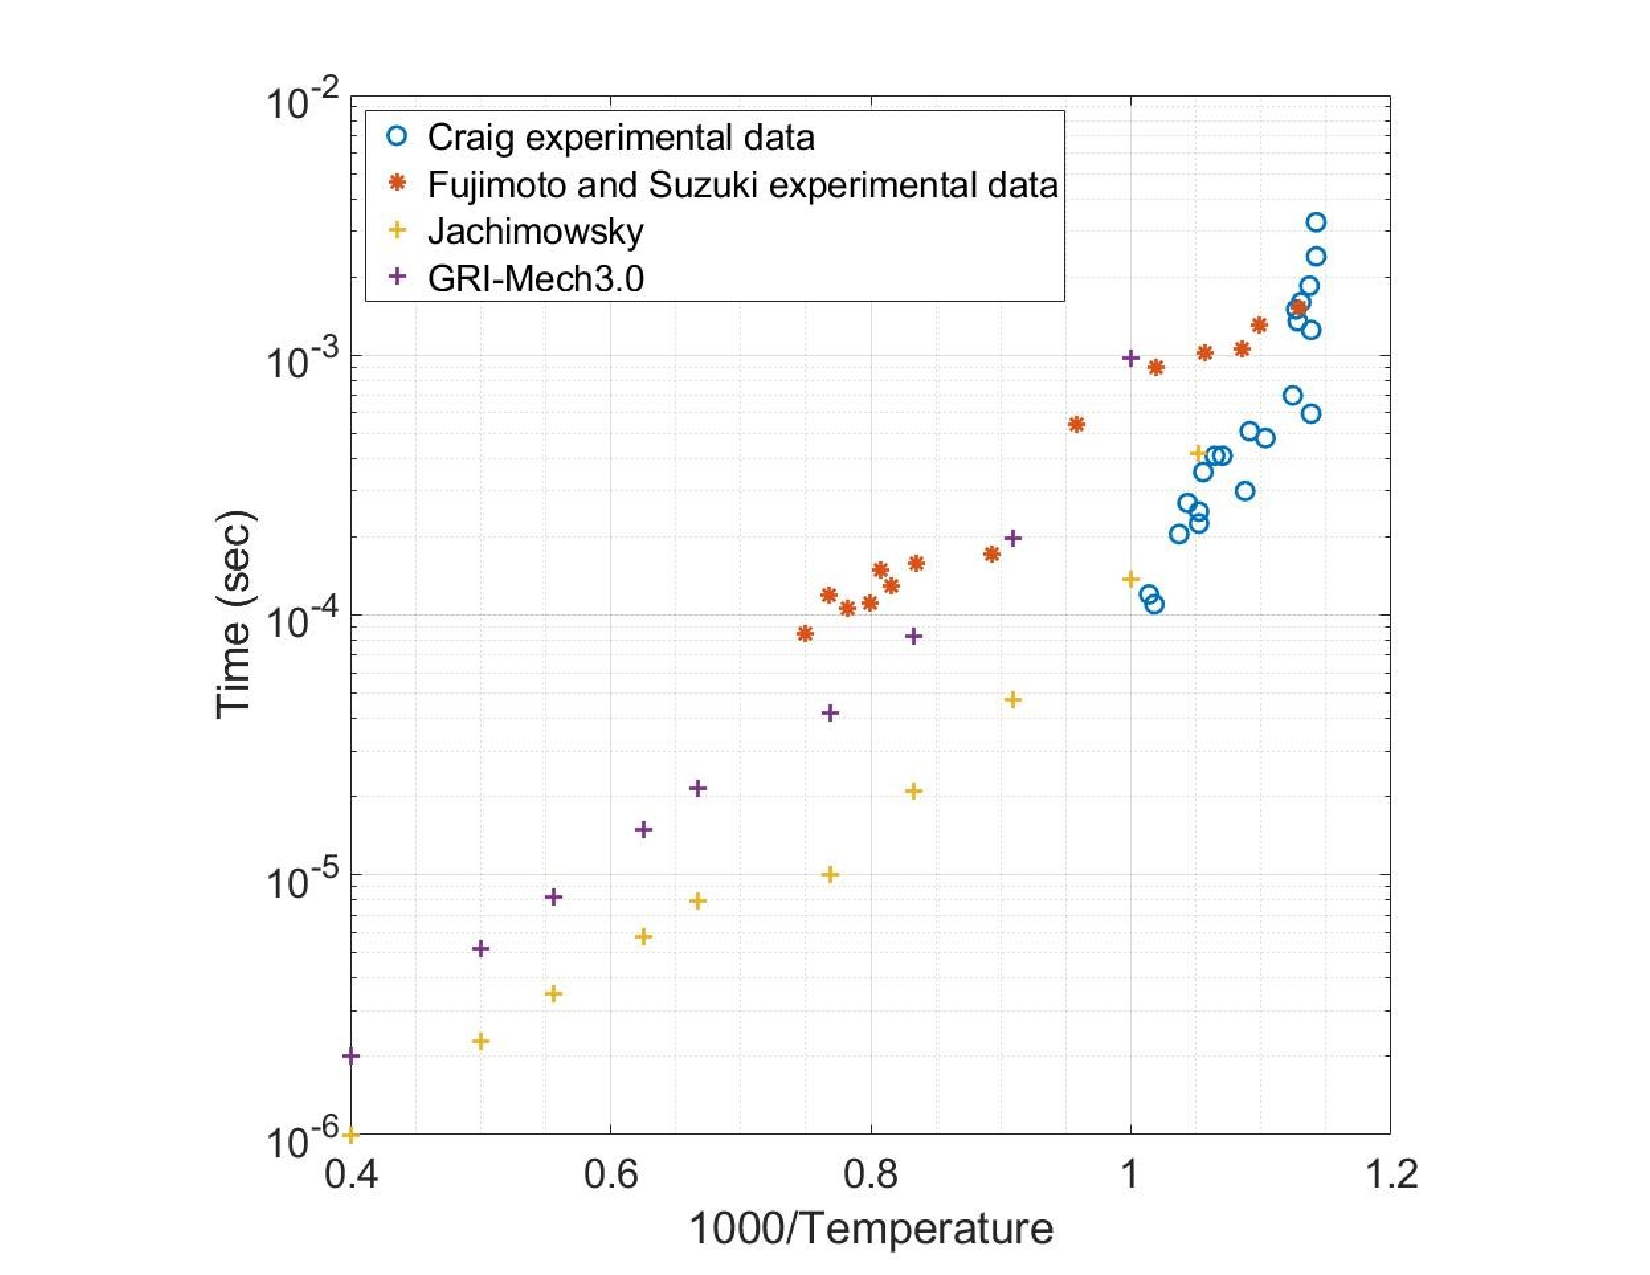
\includegraphics[width=0.49\linewidth]{5.pdf}}
\subfigure[]{\label{fig:b}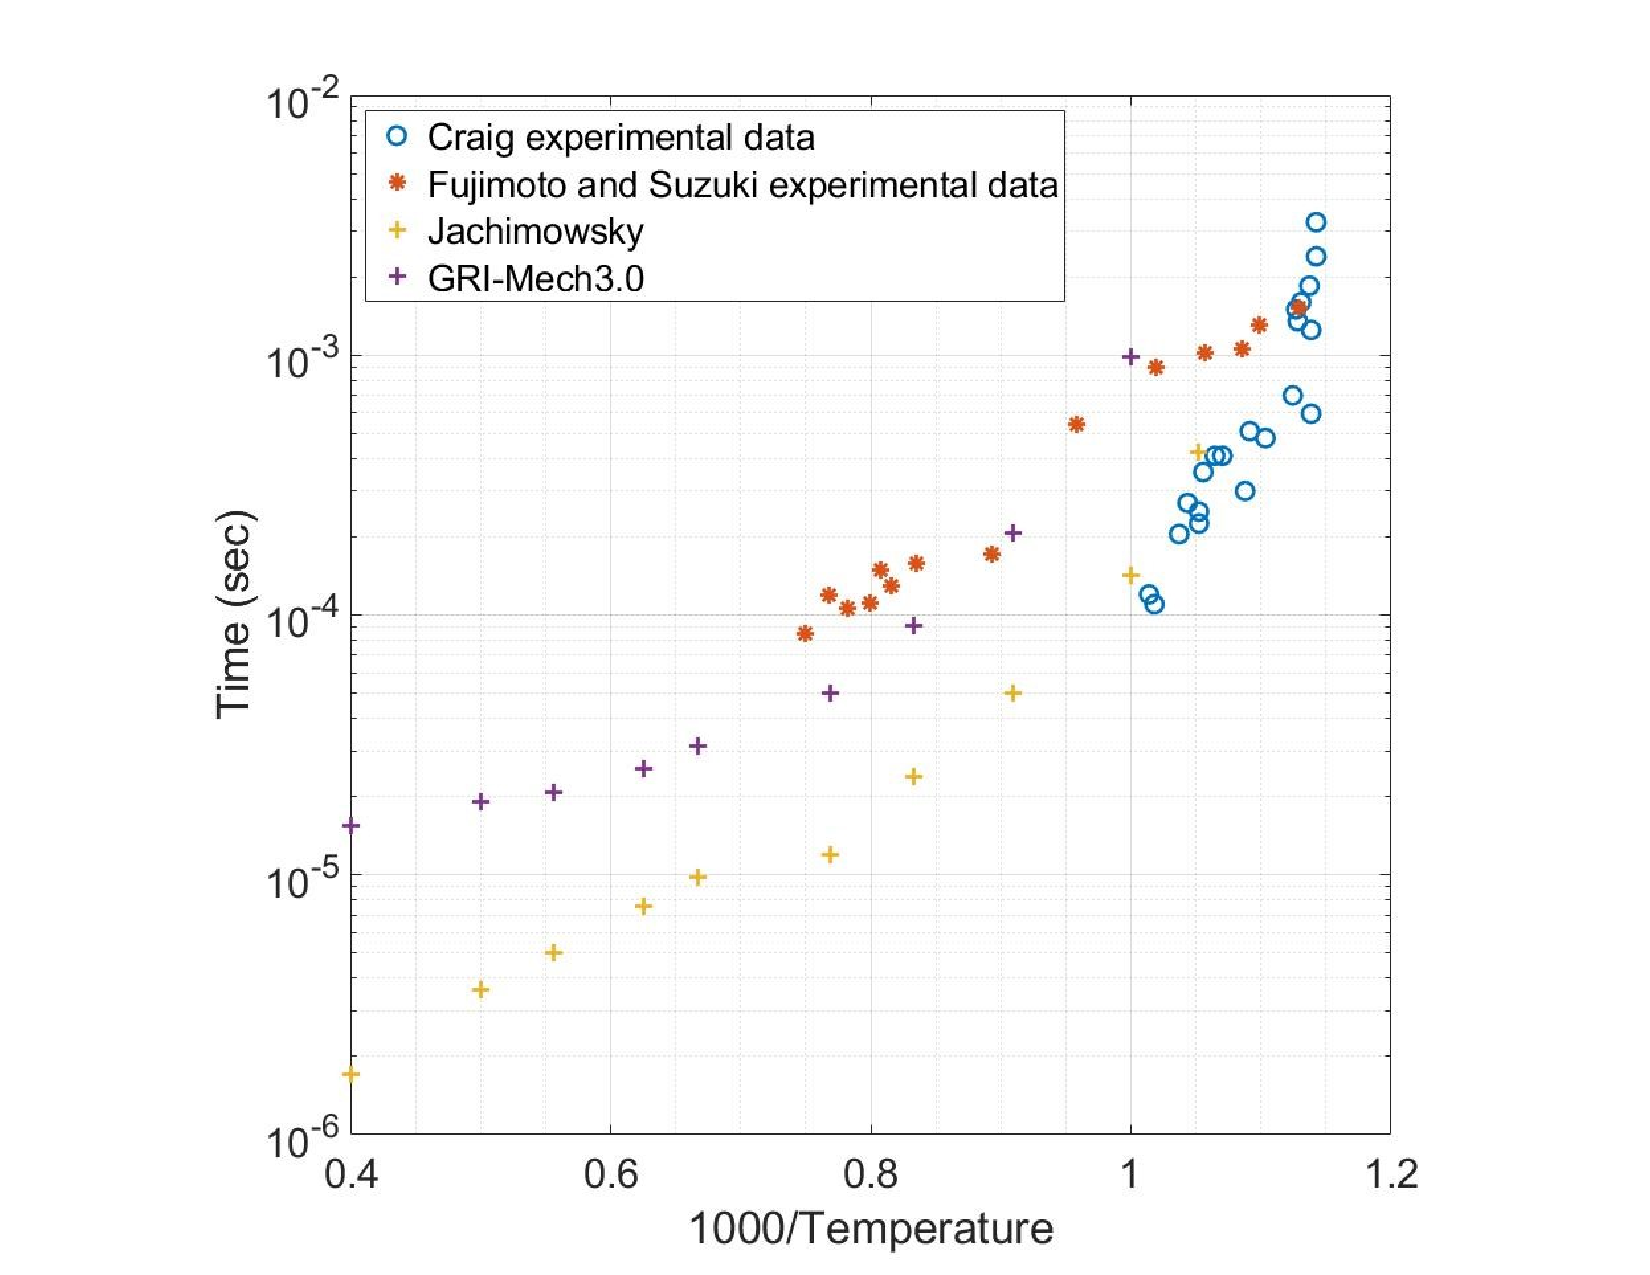
\includegraphics[width=0.49\linewidth]{50.pdf}}
\caption{Comparison of Induction time of Hydrogen - Air mixture (a) Induction time is the time taken for the temperature to go up by $5\%$ from the initial value (b) Induction time is the time taken for the temperature to go up by $50\%$ from the initial condition}
\label{fig:Induction_time_comparison}
\end{figure}






%insert a few newpages here to make sure the refs section follows the tables
~
\newpage
~
\newpage
~
\newpage
~
\newpage



\bibliographystyle{warpdoc}
\bibliography{all}


\end{document}



